% Generated by `cer p17-tables`; do not edit. Coordinates are written from the artifacts.
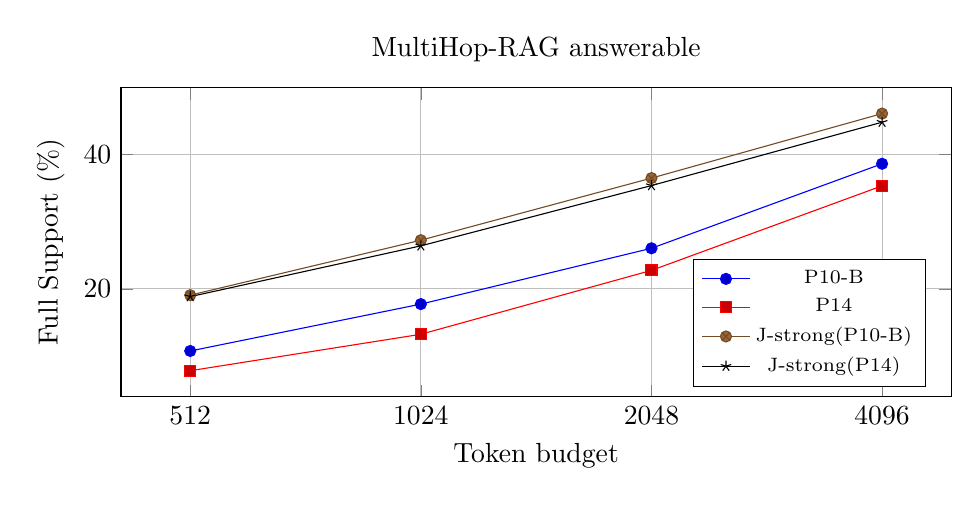
\begin{tikzpicture}
\begin{axis}[width=\columnwidth, height=5.5cm, xmode=log, log basis x=2, xtick={512,1024,2048,4096}, xticklabels={512,1024,2048,4096}, xlabel={Token budget}, ylabel={Full Support (\%)}, grid=major, legend pos=south east, legend style={font=\scriptsize}, title={MultiHop-RAG answerable}]
\addplot coordinates {(512,10.78) (1024,17.74) (2048,26.03) (4096,38.58)};
\addlegendentry{P10-B}
\addplot coordinates {(512,7.85) (1024,13.26) (2048,22.75) (4096,35.30)};
\addlegendentry{P14}
\addplot coordinates {(512,19.07) (1024,27.23) (2048,36.45) (4096,46.03)};
\addlegendentry{J-strong(P10-B)}
\addplot coordinates {(512,18.85) (1024,26.39) (2048,35.34) (4096,44.75)};
\addlegendentry{J-strong(P14)}
\end{axis}
\end{tikzpicture}
